\chapter{Simspark}

In this section you find information about the messages that are sent from the
server to the agent (perceptors) and vice versa (effectors). A description of
the perceptors and effectors can also be found in \cite{SchillingJ} (German) and \cite{Lekavy} (Slovak).

%-------------------------------------------------------------------
\section{Perceptors}
Perceptors are used to sense the environment of the agent. They are sent from
the server to each agent and contain agent specific and perceptor specific
information about the environment and the agent itself. There are perceptors
that are available to all kinds of simulations and soccer specific perceptors.

% Describe in detail, also the message format, see TEXT_INSTEAD... and Oliver's hope-1.pdf manual
% Klaus:do we have noise in perceptors?
\subsection{General Perceptors}
The perceptors described in this subsection are available to all types of
simulation. In other words they are not specific to the soccer environment.

\subsubsection{GyroRate Perceptor}
The gyro rate perceptor delivers information about the orientation of a body.
Currently only the upper torso contains a gyro perceptor.
The message contains the GYR identifier, the name of the body to which the gyro
perceptor belongs and three rotation angles. These angles describe the
orientation of the body with respect to the global coordinate system.
\begin{itemize}
	\item[Message format:] \texttt{(GYR (n <name>) (rt <x> <y> <z>))}
	\item[Example message:] \texttt{(GYR (n torso) (rt 0.01 0.07 0.46))}
\end{itemize}

%Klaus: To me it is not quite clear what the reference coordinate system is

\subsubsection{HingeJoint Perceptor}
A hinge joint perceptor receives information about the angle of the
correponding single axis hinge joint. It contains the identifier HJ, the name
of the perceptor (see table \ref{table:perceptorNames}) and the position angle of the axis. Zero
degrees corresponds to straightly allinged bodies. A hinge joint is displayed
in figure \ref{ode:hingejoint}. 

\begin{figure}[htbp]
  \begin{center}
	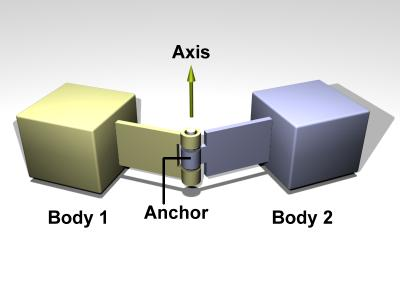
\includegraphics[scale=0.6]{fig/HingeJoint.png}
    \caption{Hinge Joint (\cite{ODEManual})}
    \label{ode:hingejoint}
  \end{center}
\end{figure}
%klaus: What is the zero degree position, is the above correct?
\begin{itemize}
	\item[Message format:] \texttt{(HJ (n <name>) (ax <ax>))}
	\item[Example message:] \texttt{(HJ (n laj3) (ax -1.02))}
\end{itemize}

\subsubsection{UniversalJoint Perceptor}
A universal joint perceptor receives information about the two angles of the
correponding two axis universal joint. It contains the identifier UJ, the name
of the perceptor (see table \ref{table:perceptorNames}) and the position angles of the two axis.
Zero degrees corresponds to straightly allinged bodies. A universal joint is
displayed in figure \ref{ode:universaljoint}. 
\begin{figure}[htbp]
  \begin{center}
	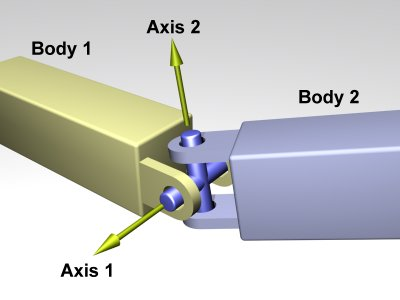
\includegraphics[scale=0.6]{fig/UniversalJoint.png}
    \caption{Universal Joint (\cite{ODEManual})}
    \label{ode:universaljoint}
  \end{center}
\end{figure}
 
\begin{itemize}
	\item[Message format:] \texttt{(UJ (n <name>) (ax1 <ax1>) (ax2 <ax2>))}
	\item[Example message:] \texttt{(UJ (n laj1\_2) (ax1 -1.32) (ax2 2.00))}
\end{itemize}

\subsection{Soccer Perceptors}
The following perceptors are soccer specific and only available in the soccer
simulation.

\subsubsection{Vision Perceptor}
Your robots possess a special omnicam with some smart image processing
software attached :). If using the regular visionperceptor, Robots
have a 360 degrees view. With the RestrictedVisionPerceptor (which
became the default in version 0.5), the view field of the robot is
restricted to 90 degrees (this is of course configurable in
rcssserver3D.rb). The direction of the view (pan and tilt) can be
changed with the pantilt effector. The camera can pan to any angle
(the initial 0 degrees pan direction is the direction towards the
opponent side), and tilt around the horizontal plane.

The VisionPerceptor delivers lists of seen objects, where objects are
either others robots, the ball, or markers on the field. Currently
there are 8 markers on the field: one at each corner point of the
field and one at each goal post.

With each sensed object you get:

\begin{itemize}
  \item The distance between the player and the object.
  \item The angle in the horizontal plane. Zero degree always points to the
opponent goal.
  \item The latitudal angle. Here zero degree means horizontal. 
\end{itemize}

Contrary to 2D soccer simulation, the vision system does not deliver
object velocities. Objects can be occluded by other objects (this is
not completely implemented yet). All distances and angles are given
relative to the camera position. The camera is currently located at
the center of the robot.
% Klaus: where is it in humanoid league

The noise parameters of the vision system are as follows:
\begin{itemize}
  \item A small calibration error is added to the camera position. For each
  axis, the error is uniformly distributed between -0.005 m and 0.005 m. The
  error is calculated once and remains constant during the complete match.
  \item Dynamic noise normally distributed around 0.0
  + distance error:  sigma = 0.0965
  + angle error (x-y plane): sigma = 0.1225
  + angle error (latitudal): sigma = 0.1480
\end{itemize}

A vision message is started with See followed by the visible objects.
Possible objects are:
\begin{itemize}
	\item[Flags:] The marker flags on the field corners F1L, F1R, F2L, F2R
	\item[Goalposts:] The goal posts of both goals G1L, G1R, G2L, G2R. Goals and
	flags are located as shown in \ref{fig:pitch}.
	\item[Ball:] The ball B 
	\item[Players:] Players P with additional information \texttt{(team <teamname>)
	(id <playerID>)}
\end{itemize}
\begin{itemize}
	\item[Message format:] \texttt{(See (<name> (pol <distance> <angle1>
	<angle2>)) (P (team <teamname>) (id <playerID>) (pol <distance> <angle1> <angle2>)))}
	\item[Example message:] \texttt{(See (F1L (pol 19.11 111.69 -9.57)) (F2L (pol 
	16.41 -115.88 -11.15)) (F1R (pol 46.53 22.04 -3.92)) (F2R (pol 45.49 -18.74
	-4.00)) (G1L (pol 9.88 139.29 -21.07)) (G2L (pol 8.40 -156.91 -25.00)) (G1R
	(pol 43.56 7.84 -4.68)) (G2R (pol 43.25 -4.10 -4.71)) (B (pol 18.34 4.66
	-9.90)) (P (team RoboLog) (id 1) (pol 37.50 16.15 -0.00)))}
\end{itemize}
% What about the Restricted Vision Perceptor?
% The current soccer bot seems not to use it, still experimental/unsupported?

\subsubsection{GameState Perceptor}
The GameStatePerceptor contains information of the current play time which
starts from zero at kickoff of either half. It also contains the current game status.
The first percept you get from this perceptor additionally tells you about some
of the game variables, like ball weight and field size.

All other percepts start with GS and contain the current simulation time as a
float value passed in seconds and the playmode. Possible
playmodes are "BeforeKickOff", "KickOff\_Left", "KickOff\_Right",
"PlayOn", "KickIn\_Left", "KickIn\_Right", "corner\_kick\_left",
"corner\_kick\_right", "goal\_kick\_left", "goal\_kick\_right",
"offside\_left", "offside\_right", "GameOver", "Goal\_Left",
"Goal\_Right", "free\_kick\_left", "free\_kick\_right", "unknown". For an
up to date list of all playmodes refer to (./plugin/soccer/soccertypes.h)

\begin{itemize}
	\item[Message format:] \texttt{(GS (t <time>) (pm <playmode>))}
	\item[Example message:] \texttt{(GS (t 0.00) (pm BeforeKickOff))}
\end{itemize}

\subsubsection{AgentState Perceptor}
%klaus: is this old version only? if not is TEXT_INSTEAD_OF_A_MANUAL still
% correct?
\begin{itemize}
	\item[Message format:] \texttt{}
	\item[Example message:] \texttt{}
\end{itemize}
\subsubsection{Hear Perceptor}
%klaus: is this old version only? if not is TEXT_INSTEAD_OF_A_MANUAL still
% correct?
\begin{itemize}
	\item[Message format:] \texttt{}
	\item[Example message:] \texttt{}
\end{itemize}
\subsubsection{Touch Perceptor}
%klaus: is this old version only? if not is TEXT_INSTEAD_OF_A_MANUAL still
% correct?
\begin{itemize}
	\item[Message format:] \texttt{}
	\item[Example message:] \texttt{}
\end{itemize}
\subsubsection{ForceResistance Perceptor}
This perceptor informs about the force that acts on a body. Currently, it is
available for the left and the right foot (lf, rf).
After FRP and the name of the body it contains two vectors that indicate the
point on the body to which the force applies and the force vector itself.
%klaus: how exactly does this work, what is the unit?
%klaus: is this general or soccer specific?
\begin{itemize}
	\item[Message format:] \texttt{(FRP (n <name>) (c <px> <py> <pz>) (f <fx> <fy>
	<fz>))}
	\item[Example message:] \texttt{(FRP (n lf) (c -0.14 0.08 -0.05) (f 1.12 -0.26
	13.07))}
\end{itemize}

%-------------------------------------------------------------------
\section{Effectors/Actuators}
Effectors are used to act within the simulation. They are sent to the server
to change the game state accordingly. There are effectors that are available to
all kinds of simulations and soccer specific effectors.
%Klaus: do we have noise in effectors?
%Klaus: What are the minimal/maximal values to pass? What happens in case of
% errors

\subsection{General Effectors}
The effectors described in this subsection are available to all types of
simulation. In other words they are not specific to the soccer environment.

\subsubsection{Create Effector}

When an agent initially connects to the server it is invisible and
cannot take affect a simulation in any meaningful way. It only
possesses a so called CreateEffector.

An agent uses this effector to advice the server to construct it
according to a scene description file it passes as a parameter. This
file is used to construct the physical representation and all further
effectors and preceptors.
\begin{itemize}
	\item[Message format:] \texttt{(scene  <filename>)}
	\item[Example message:] \texttt{(scene rsg/agent/soccerbot056.rsg)}
\end{itemize}

After the agent representation is constructed in the server the agent
should do further simulation specific setup. For example in the soccer
simulation each agent is required to register to a team and acquire a
unique player number. For these tasks usually a special effector like
the SoccerInitEffector is used.

% Explain that these effectors are available to all simulations

\subsubsection{HingeJoint Effector}
Effector for all axis with a single degree of freedom.
The first parameter is the name of the axis. Table ??? shows a list of all
available hinge joints. The second parameter contains the change in angle of
the joint.
\begin{itemize}
	\item[Message format:] \texttt{(<name> <ax>)}
	\item[Example message:] \texttt{(lae3 5.3)}
\end{itemize}

\subsubsection{UniversalJoint Effector}
Effector for all axis with a two degrees of freedom.
The first parameter is the name of the axis. Table ??? shows a list of all
available hinge joints
The second and third parameter contain the change in angle of the two joints.
The order of the joints is the same as in the name.
\begin{itemize}
	\item[Message format:] \texttt{(<name> <ax1> <ax2>)}
	\item[Example message:] \texttt{(lae1\_2 -2.3 1.2)}
\end{itemize}

\subsection{Soccer Effectors}
The following effectors are soccer specific and only available in the soccer
simulation.

\subsubsection{Init Effector}
The init command is sent once for each agent after the create effector sent the
scene command. It registers this agent as a member of the passed team with the passed number.
All players of one team have to use the same teamname and different numbers.
If an agent sends 0 as playernumber, the number is assigned automatically by
the server to the next free number. The maximum amount of teams is two, the
maximal amount of players is currently four.
The side on which a team starts to play depends on which team connected
first.
\begin{itemize}
	\item[Message format:] \texttt{(init (unum <playernumber>)(teamname
	<yourteamname>))}
	\item[Example message:] \texttt{(init (unum 1)(teamname FHO))}
\end{itemize}

\subsubsection{Beam Effector}
The beam effector allows a player to position itself on the field before the
game starts. The x and y coordinates define the position on the field with
respect to the coordinate system of figure ???. The rot value allows to define
the rotation angle of the player. Zero degrees points to positive x axis, 90
degrees to positive y axis.
\begin{itemize}
	\item[Message format:] \texttt{(beam <x> <y> <rot>)}
	\item[Example message:] \texttt{(beam 10.0 -10.0 0.0)}
\end{itemize}

\subsubsection{Say Effector}
%klaus: is this old version only?

\subsection{Older Version Effectors}
The effectors in this subsection have been available in older versions of the
simulation and are now no longer available

\subsubsection{Drive Effector}
To use the omnidrive of the agent, you have to use the so called
"DriveEffector", which takes a cartesian vector (x y z) with a maximum
length of 100 units. The x-coordinate points towards the opponents
team side of the field, z points up. With the DriveEffector, you set a
kind of motor force, i.e. if you want to drive full speed for a while,
it is sufficient to use the DriveEffector *once*. The force you set is
applied at each simulator step until you change it again. The
DriveEffector works reliable, there is a small error for forces along
each axis (each up to 2\% of the applied force). The error is normally
distributed around 0.0.

Using the omnidrive consumes battery. You get to know of battery
states by reading the AgentStatePerceptor. If the battery is empty,
the omnidrive will stop working. It is also possible to push away
other robots. Using this feature to push away opponents is discouraged
:).

\begin{itemize}
	\item[Message format:] \texttt{(drive <x> <y> <z>)}
	\item[Example message:] \texttt{(drive 20.0 50.0 0.0)}
\end{itemize}


\subsubsection{Kick Effector}
To move the ball, you have the option of simply using the robots to
push the ball into a desired direction, or you can use the
kickeffector to kick the ball. Originally, we did not intend to create
an artificial kickeffector. However, to make use of the 3rd dimension,
this was the easiest way. It is intended to remove this kind of kick
effector in future versions (not this years' competition) in favor of
a real physical device.

The kickeffector can accelerate the ball radially away from the robot
body. The kickeffector takes an angle as first argument. This is the
latitudal angle (in degrees) for accelerating the ball. It is
restricted to a number between 0 and 50. The second argument indicates
the kicking power and this is a number between 0 and 100. It is
interpreted as the percentile of the maximum available power. The
kickeffector adds a force and a torque to the ball. This happens over
a fixed number of simulation steps. Currently 10 cycles are used. This
corresponds to 1/10s simulation time. To kick the ball, the ball has
to be very close to the robot, i.e. it has to be within the so called
kickable margin of the player. Currently 0.04m are configured.

You cannot change the kicking angle in the horizontal plane. This
means that you have to move the robot so that it can kick into the
desired direction. Right now, the kickeffector is not very strong,
because something like an offside rule is missing. It should also not
be possible to move other robots by kicking the ball against them
anymore. (at least not very much :) Like the DriveEffector, the
kickeffector does only work if the robot touches the soccer field.

The kickeffector noise has the following parameters: 
\begin{itemize}
\item The angle error in the x-y plane is quite low and normally distributed
around 0.0 with sigma = 0.02.
\item The latitudal angle error is normally distributed around 0.0. This
angle error is low with sigma = 0.9 at both extreme positions, i.e. 0
and at 50 degrees. Towards the middle of the range the angle error
gets higher with sigma up to 4.5.
\item The kick power error is normally distributed around 0.0 with sigma =
0.4
\end{itemize}

\begin{itemize}
	\item[Message format:] \texttt{(kick <angle> <power>)}
	\item[Example message:] \texttt{(kick 20.0 80.0)}
\end{itemize}

\subsubsection{Catch Effector}
The goalie (agent number 1) is the only player with the ability to
catch a ball. The goalie can catch the ball in play mode 'playe\_on',
if the ball is inside the penalty area and close to the robot, i.e. it
has to be within the so called catch margin of the player. The current
value of catch margin is 2 meters.

The catcheffector puts the ball in front of the goalie on the ground
and moves players away that are closer than 2 meters to the goalie by
5 meters.

\begin{itemize}
	\item[Message format:] \texttt{(catch)}
	\item[Example message:] \texttt{(catch)}
\end{itemize}

%----------------------------------------------------------------------
\section{Simulation Update Loop}

% I think people want to know how this works, maybe we can give an overview here and go into more detail in the developer manual? What do you think?

SimSpark implements a simple internal event model that immediately
executes every action received from an agent. It does not try to
compensate any network latency or compensate for different computing
resources available to the connected agents.

A consequence is that SimSpark currently does not guarantee that
events are reproducible. This means repeated simulations may have a
different outcome, depending on network delays or load variations on
the machines hosting the agents and the server.

A benefit of the simple structure however are speed gains that make it
interesting for machine learning tasks as in these setups an often
large number of different agent and simulation configurations are
repeatedly tested.

Further the SimSpark main loop is highly customizable as it is
entirely build upon plugins we call simcontrol nodes. Simcontrol nodes
are registered to the simulation server. They act in response to
control events. The simulation server repeatedly generates these as it
executes an abstracted the main loop.

The event types are an 'init' event once when the simulation server
starts and a 'done' event on shutdown. The main then loop cycles
repeatedly through the 'start cycle', 'sense agent', 'act agent' and
'end cycle' events.

Apart from generating control events the simulation server advances
the simulation time passed in the last cycle. Depending on its
configuration it either does this in discrete time quanta or in one
single step.

A simcontrol node further can take responsibility for the time
measurement, for example to synchronize the simulation time with the
real time used to render the scene.  Otherwise the simulation is
stepped a fixed time step as often as possible.

In this way all management tasks are implemented as plugins to the
simulation server. This involves the agent management, monitor
management, rendering, mouse and keyboard input and network code.

This setup allows us to configure the simulation at runtime as either
a monolithic application that does both simulation and rendering or as
a dedicated simulation server that defers rendering to a remote
monitor application.

\subsection{Single-threaded Timer}

In the singled-threaded mode, the main loop cycles repeatedly through
the `start cycle', `sense agent', `act agent' and `end cycle' events(
see \autoref{fig:single-thread-sd}). There are two noticeable details:
\begin{itemize}
\item Each cycle duration is 20ms, if the simulation is fast than real
  time, it will wait; otherwise, if the simulation is very slow, it
  will run many physics updates once without interaction with agents.
  If the simulation is very slow, it will give up to catch up the real
  time and print warning. So you may have problem while the computer
  is not fast enough.
\item The `act agent' event is followed after `sense agent', the
  action which the agent send according to $n^{th}$ cycle will be
  realized in the $(n+1)^{th}$ cycle, i.e. the action has been delayed
  one cycle. See for \autoref{fig:synchronization} explanation.
\end{itemize}

\begin{figure}[htp]
  \centering
  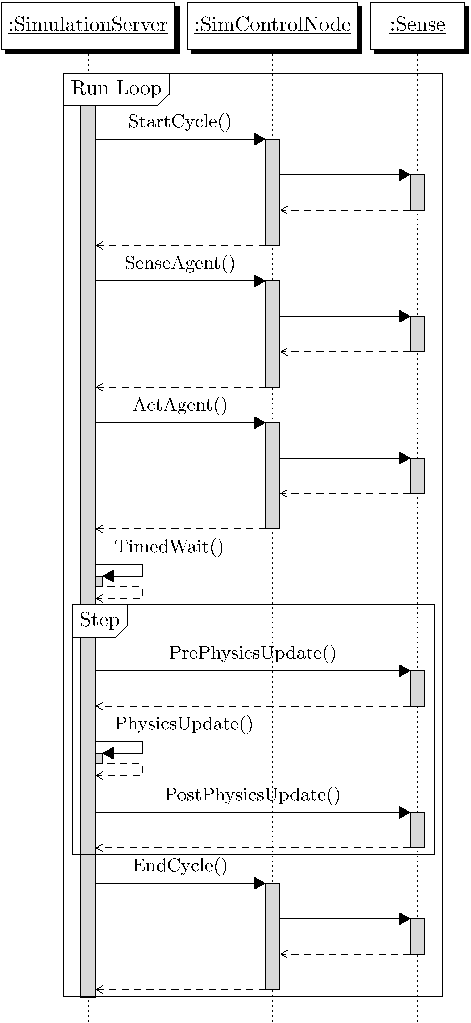
\includegraphics[height=0.6\textheight]{fig/serverSingleThreadLoop}
  \caption{Single-threaded loop UML sequence diagram}
  \label{fig:single-thread-sd}
\end{figure}

\begin{figure}[htp]
  \centering
  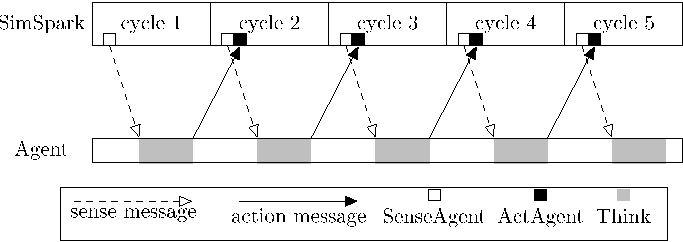
\includegraphics[width=0.8\textwidth]{fig/synchronization}
  \caption{Synchronization between SimSpark and agent}
  \label{fig:synchronization}
\end{figure}

\subsection{Multi-threaded Timer}
In modern time, computers have more than one CPU or dual cores in one
CPU. This improve the performance greatly, but only the multi-threaded
program can benefit. SimSpark has an experimental multi-threaded
running loop, it can be switched on simply by change the
\texttt{simulationServer.setMultiThreads(false)} to
\texttt{simulationServer.setMultiThreads(true)} in the
\texttt{spark.rb} file.

The implementation of multi-threaded loop is based on two conditions.
First, every SimControlNode response for different parts of the
simulation, they perform one by one in the singled-threaded mode, but
they can run in parallel. Second, there is a active scene which stores
the whole simulation data in a tree. The physics engine and
SimControlNode interact through the active scene. As we know, the
physics computation is the most time-consuming, and the physics engine
does not need to access the active scene during physics computation.
So the physics computation and SimControlNodes can run in parallel. At
last, we get the multi-threaded simulation loop as
\autoref{fig:multi-thread-sd}. Note that the agent's action are also
delayed one cycle in the multi-threaded loop.
\begin{figure}[htp]
  \centering
  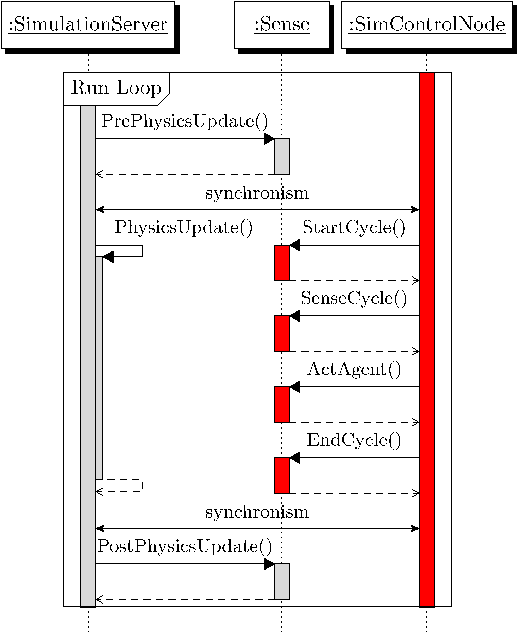
\includegraphics[height=0.5\textheight]{fig/serverMultiThreadLoop}
  \caption{Multi-threaded loop UML sequence diagram, note that
    each SimControlNode runs in separated thread.}
  \label{fig:multi-thread-sd}
\end{figure}

%----------------------------------------------------------------------
\section{Setup Scripts}

% describe purpose of scripts in ~/.rcssserver3d/]

% kerosin.rb for rendering configuration of simspark

%%% Local Variables: 
%%% mode: latex
%%% TeX-master: "user-manual"
%%% End: 
